\chapter{HASIL DAN PEMBAHASAN}
\label{chap:hasilpembahasan}

Pada bab ini dipaparkan hasil dari eksperimen yang dilakukan pada penelitian ini.
Hasil dari training berupa \emph{mean episode rewards} dari agen \emph{attacker} dan agen \emph{defender},
waktu training, rerata waktu inferensi, rerata waktu proses \emph{actions}, rerata waktu \emph{environment} menunggu,
rerata waktu pemrosesan observasi mentah, dan presentase penggunaan CPU serta RAM.

Hasil dari evaluasi berupa performa algoritma jika dilawankan dengan generasi sebelum dan sesudahnya,
serta evaluasi performa algoritma dalam skenario \emph{environment} yang berbeda berupa area lebih besar
(16x16).

\section{Hasil Training}

Dalam eksperimen RL, hal yang paling penting untuk diperhatikan adalah rerata \emph{rewards} (\emph{mean episode rewards}) yang didapatkan oleh agen
selama training. Performa agen RL dapat diukur dengan seberapa banyak reward yang telah didapatkan oleh agen.
Dari eksperimen yang telah dilakukan, didapatkan \emph{mean episode rewards} untuk kedua agen dengan keempat algoritma yang diuji coba.
\emph{Mean episode rewards} merupakan rerata nilai \emph{rewards} yang didapatkan oleh agen selama satu episode.

\subsection{Attacker Mean Episode Rewards}

\begin{figure}[H]
  \centering
    % Nama dari file gambar yang diinputkan
    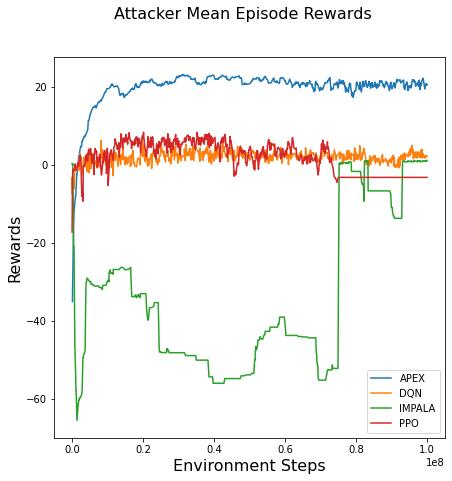
\includegraphics[scale=0.52]{gambar/attacker_reward_mean.jpg}
    % Keterangan gambar yang diinputkan
    \caption{Grafik menunjukan \emph{mean episode rewards} dari agen \emph{attacker}.
    Biru: APE-X DQN, oranye: DQN, hijau: IMPALA, merah: PPO}
    % Label referensi dari gambar yang diinputkan
    \label{fig:attackerMeanEpisodeGraph}
\end{figure}

Dari grafik \ref{fig:attackerMeanEpisodeGraph}, APE-X DQN merupakan algoritma yang paling baik,
jauh di atas algoritma lain. APE-X DQN mencapai nilai 20 poin sekitar pada 1.5 \emph{environment steps}.
APE-X DQN berkonvergensi di sekitar nilai 20 poin ini sebelum 2 juta \emph{environment steps}.
Mengingat 20 poin merupakan nilai \emph{reward} ketika agen \emph{attacker} menghancurkan kota,
agen \emph{attacker} APE-X DQN secara konsisten telah menyelesaikan tujuan tersebut.

Algoritma lain jauh dibawah performa APE-X DQN. Algoritma DQN selalu di bawah 5 poin dan tidak meningkat secara signifikan.
Algoritma PPO mencapai nilai 5 poin pada sekitar 1.5 juta \emph{environment steps}, akan tetapi menurun setelah 5 juta
\emph{environment steps}. PPO juga mengalami \emph{flatline} dimana secara tiba tiba algoritma tersebut
tidak mengalami peningkatan atau penurunan nilai \emph{rewards} pada sebelum 8 juta \emph{environment steps}
sampai akhir sesi. PPO merupakan algoritma terburuk pada grafik ini. IMPALA merupakan algoritma yang paling tidak stabil pada grafik ini.
Nilai \emph{mean episode rewards} agen \emph{attacker} IMPALA selalu di bawah -20 poin sampai
sekitar sebelum 8 juta \emph{environment steps} dimana IMPALA melonjak ke nilai 0 poin.
Nilai poin negatif dari IMPALA hanya bisa dicapai jika \emph{unit} agen \emph{attacker} mencoba untuk keluar
dari batas \emph{environment} secara terus menerus.

\subsection{Defender Mean Episode Rewards}

\begin{figure}[H]
  \centering
    % Nama dari file gambar yang diinputkan
    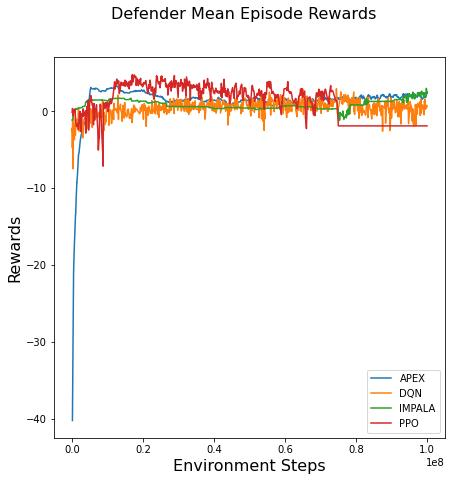
\includegraphics[scale=0.52]{gambar/defender_reward_mean.jpg}
    % Keterangan gambar yang diinputkan
    \caption{Grafik menunjukan \emph{mean episode rewards} dari agen \emph{defender}.
    Biru: APE-X DQN, oranye: DQN, hijau: IMPALA, merah: PPO}
    % Label referensi dari gambar yang diinputkan
    \label{fig:defenderMeanEpisodeGraph}
\end{figure}

Perubahan nilai \emph{rewards} algoritma dalam grafik \ref{fig:defenderMeanEpisodeGraph} jauh lebih stabil.
Hal ini disebabkan karena nilai \emph{general reward} yang diterima oleh agen \emph{defender} tidak memiliki varian yang tinggi,
dibandingkan dengan agen \emph{attacker} yang memerima 20 poin ketika menghancurkan kota.

APE-X DQN memulai dengan -40 poin akan tetapi secara cepat melonjak ke atas 2 poin.
Sama dengan di grafik \ref{fig:attackerMeanEpisodeGraph}, APE-X DQN merupakan algoritma paling stabil.
APE-X DQN juga salah satu algoritma dengan performa terbaik, bersebelahan dengan IMPALA.

DQN tidak berhasil melakukan konvergensi dengan baik dan nilainya tidak stabil sampai akhir sesi.
PPO juga merupakan algoritma terburuk pada grafik ini. Keadaan \emph{flatline} sama yang dialami PPO pada grafik
\ref{fig:attackerMeanEpisodeGraph} juga dapat dilihat disini.

\subsection{Waktu dan Pemakaian Resource Algoritma}

\begin{table}[H]
  \centering
  \caption{Training, Inference, Processing Time, and Resource Usage}
  \label{table:timeAndResourceSpent}
  \begin{tabular}{|l|l|l|l|l|}
      \hline
      \textbf{Metrics}                                                            & \textbf{APE-X DQN} & \textbf{DQN}     & \textbf{PPO}     & \textbf{IMPALA}  \\ \hline
      \begin{tabular}[c]{@{}l@{}}Total Training \\ Time\end{tabular}          & 1d 17h             & 8d 7h            & 3d 3h             & 23h     \\ \hline
      \begin{tabular}[c]{@{}l@{}}Mean Inference \\ (ms)\end{tabular}          & 3.406     & 9.191   & 2.446   & 1.862   \\ \hline
      \begin{tabular}[c]{@{}l@{}}Mean Action \\ Processing (ms)\end{tabular}  & 0.06758   & 0.07171 & 0.05702 & 0.05636 \\ \hline
      \begin{tabular}[c]{@{}l@{}}Mean Environment \\ Wait (ms)\end{tabular}   & 0.457     & 0.4237  & 0.414   & 0.4119  \\ \hline
      \begin{tabular}[c]{@{}l@{}}Mean Raw Obs \\ Processing (ms)\end{tabular} & 0.3512    & 0.2834  & 0.2363  & 0.2143  \\ \hline
      RAM Utilization                                                         & 82.3\%    & 38.82\% & 36.1\%  & 33.2\%  \\ \hline
      CPU Utilization                                                         & 79.95\%   & 40.78\% & 39.63\% & 63.51\% \\ \hline
  \end{tabular}
\end{table}

Tabel \ref{table:timeAndResourceSpent} menunjukan bahwa IMPALA merupakan algoritma tercepat
untuk menyelesaikan 10 juta \emph{environment step} dengan \emph{total training time} selama
23 jam. APE-X DQN mengikuti IMPALA tidak jauh setelahnya dengan \emph{total training time}
selama 1 hari 7 jam (30 jam). PPO memerlukan waktu lebih dari 3x lebih lama dengan \emph{total training time}
sebesar 3 hari 3 jam (75 jam). DQN merupakan algoritma terlama yang memerlukan 8 hari 7 jam (199 jam).

IMPALA juga merupakan algoritma tercepat dalam inferensi dengan nilai \emph{mean inference} sebesar
1.862 ms. PPO merupakan algoritma tercepat kedua dengan \emph{mean inference} sebesar 2.446 ms walaupun \emph{total
training time} PPO lebih lambat dari APE-X DQN, APE-X DQN berada di setelah PPO dengan \emph{mean inference}
sebesar 3.406 ms. DQN merupakan algoritma terlama dalam melakukan inferensi dengan 9.191 ms.
\emph{Metrics} lainnya seperti \emph{mean action processing}, \emph{mean environment wait}, dan \emph{mean raw obs processing}
tidak berbeda jauh antara satu algoritma dengan algoritma lainnya.

Pada penggunaan RAM dan CPU, APE-X DQN merupakan algoritma yang menggunakan CPU dan RAM terbanyak
dengan penggunaan CPU sebesar 79.95\% dan RAM sebesar 82.3\%. Hal ini disebabkan oleh penggunaan CPU
APE-X DQN yang menggunakan seluruh 8 \emph{cores} dibandingkan algoritma lain yang menggunakan 4 \emph{cores}
dengan jumlah \emph{workers} yang sama (3 \emph{workers}). IMPALA merupakan algoritma DRL
terdistribusi lainnya yang menggunakan CPU terbanyak setelah APE-X DQN dengan penggunaan sebesar
63.51\%. Akan tetapi penggunaan RAM dari IMPALA jauh lebih minim dengan penggunaan sebesar 33.2\%.
PPO dan DQN menggunakan CPU dan RAM sama banyaknya dengan penggunaan CPU sebesar 39-40\% dan RAM
sebesar 36-39\%.

\section{Hasil Evaluasi}
Setelah dilakukan \emph{training}, terdapat dua macam evaluasi yang dilakukan.
Evaluasi antar generasi algoritma dan evaluasi dengan \emph{environment} yang lebih luas.
Hasil dari kedua evaluasi merupakan \emph{rewards} yang didapatkan oleh agen pada setiap generasi algoritma.

\subsection{Hasil Evaluasi Antar Generasi Algoritma}

\begin{table}[H]
  \centering
  \caption{Evaluasi Antar Generasi DQN}
  \label{table:dqnVersusResult}
  \begin{tabular}{|c|c|c|c|}
  \hline
  \textbf{\begin{tabular}[c]{@{}c@{}}Attacker Agent\\ Generation\end{tabular}} & \textbf{\begin{tabular}[c]{@{}c@{}}Defender Agent\\ Generation\end{tabular}} & \textbf{\begin{tabular}[c]{@{}c@{}}Attacker Mean\\ Episode Rewards\end{tabular}} & \textbf{\begin{tabular}[c]{@{}c@{}}Defender Mean\\ Episode Rewards\end{tabular}} \\ \hline
  \multirow{4}{*}{1}                                                           & 1                                                                            & -80.15                                                                           & -6.53                                                                            \\ \cline{2-4} 
                                                                               & 2                                                                            & -71.4                                                                            & -15.75                                                                           \\ \cline{2-4} 
                                                                               & 3                                                                            & -79.617                                                                          & -53.08                                                                           \\ \cline{2-4} 
                                                                               & 4                                                                            & -82.76                                                                           & -37.38                                                                           \\ \hline
  \multirow{4}{*}{2}                                                           & 1                                                                            & -0.46                                                                            & -18.46                                                                           \\ \cline{2-4} 
                                                                               & 2                                                                            & -0.56                                                                            & -13.53                                                                           \\ \cline{2-4} 
                                                                               & 3                                                                            & -0.41                                                                            & -48.12                                                                           \\ \cline{2-4} 
                                                                               & 4                                                                            & -0.66                                                                            & -27.16                                                                           \\ \hline
  \multirow{4}{*}{3}                                                           & 1                                                                            & -0.72                                                                            & -16.53                                                                           \\ \cline{2-4} 
                                                                               & 2                                                                            & -1.98                                                                            & -13.38                                                                           \\ \cline{2-4} 
                                                                               & 3                                                                            & -1.68                                                                            & -46.59                                                                           \\ \cline{2-4} 
                                                                               & 4                                                                            & -2.6                                                                             & -25.1                                                                            \\ \hline
  \multirow{4}{*}{4}                                                           & 1                                                                            & -0.71                                                                            & -15.78                                                                           \\ \cline{2-4} 
                                                                               & 2                                                                            & -0.65                                                                            & -11.86                                                                           \\ \cline{2-4} 
                                                                               & 3                                                                            & -1.30                                                                            & -48.36                                                                           \\ \cline{2-4} 
                                                                               & 4                                                                            & -0.52                                                                            & -28.56                                                                           \\ \hline
  \end{tabular}
\end{table}

Pada algoritma DQN, performa antar generasi agen \emph{attacker} memmiliki nilai \emph{mean episode rewards} yang mirip, kecuali generasi pertama.
Performa agen \emph{attacker} generasi 1 jauh dibawah performa generasi-generasi selanjutnya.
Ini merupakan salah satu dampak penggunaan \emph{epsilon greedy} dalam algoritma DQN.
Algoritma DQN akan melakukan aksi secara acak pada saat \emph{training} untuk melakukan eksplorasi.
Generasi pertama akan sering melakukan eksplorasi untuk mencari nilai \emph{Q-value} yang optimal
Generasi-generasi setelahnya melakukan \emph{exploitation} akan eksplorasi yang sudah dilakukan oleh generasi sebelumnya.
Untuk agen \emph{defender}, generasi 3 merupakan generasi yang paling buruk.
Generasi ke 3 memiliki nilai paling rendah saat melawan generasi manapun.

\begin{table}[H]
  \centering
  \caption{Evaluasi Antar Generasi APEX DQN}
  \label{table:apexDqnVersusResult}
  \begin{tabular}{|c|c|c|c|}
  \hline
  \textbf{\begin{tabular}[c]{@{}c@{}}Attacker Agent\\ Generation\end{tabular}} & \textbf{\begin{tabular}[c]{@{}c@{}}Defender Agent\\ Generation\end{tabular}} & \textbf{\begin{tabular}[c]{@{}c@{}}Attacker Mean\\ Episode Rewards\end{tabular}} & \textbf{\begin{tabular}[c]{@{}c@{}}Defender Mean\\ Episode Rewards\end{tabular}} \\ \hline
  \multirow{4}{*}{1}                                                           & 1                                                                            & -14.33                                                                                                & -56.00                                                                                                \\ \cline{2-4} 
                                                                              & 2                                                                            & -25.50                                                                                                & -29.14                                                                                                \\ \cline{2-4} 
                                                                              & 3                                                                            & -11.74                                                                                                & -24.78                                                                                                \\ \cline{2-4} 
                                                                              & 4                                                                            & -16.30                                                                                                & 3.25                                                                                                  \\ \hline
  \multirow{4}{*}{2}                                                           & 1                                                                            & -6.88                                                                                                 & -49.60                                                                                                \\ \cline{2-4} 
                                                                              & 2                                                                            & -65.80                                                                                                & -53.00                                                                                                \\ \cline{2-4} 
                                                                              & 3                                                                            & -2.66                                                                                                 & 1.65                                                                                                  \\ \cline{2-4} 
                                                                              & 4                                                                            & -2.19                                                                                                 & -3.21                                                                                                 \\ \hline
  \multirow{4}{*}{3}                                                           & 1                                                                            & 4.54                                                                                                  & -52.10                                                                                                \\ \cline{2-4} 
                                                                              & 2                                                                            & 7.02                                                                                                  & -7.23                                                                                                 \\ \cline{2-4} 
                                                                              & 3                                                                            & 6.34                                                                                                  & 2.11                                                                                                  \\ \cline{2-4} 
                                                                              & 4                                                                            & 5.50                                                                                                  & 3.26                                                                                                  \\ \hline
  \multirow{4}{*}{4}                                                           & 1                                                                            & 13.80                                                                                                 & -20.82                                                                                                \\ \cline{2-4} 
                                                                              & 2                                                                            & 10.50                                                                                                 & -2.00                                                                                                 \\ \cline{2-4} 
                                                                              & 3                                                                            & 12.20                                                                                                 & 2.55                                                                                                  \\ \cline{2-4} 
                                                                              & 4                                                                            & 11.70                                                                                                 & 3.11                                                                                                  \\ \hline
  \end{tabular}
\end{table}

Algoritma APEX DQN memiliki awal yang mirip dengan DQN, dimana nilai \emph{mean episode rewards} sangat kecil pada generasi awal.
Hal ini karena APEX DQN juga menggunakan \emph{epsilon greedy} untuk eksplorasi dan eksploitasi nilai \emph{Q-value}.
Namun, dapat dilihat bahwa nilai \emph{episode mean rewards} kedua agen meningkat pada setiap generasi.
Agen \emph{attacker} mampu mendapatkan nilai di atas sepuluh pada generasi ke empat.

\begin{table}[H]
  \centering
  \caption{Evaluasi Antar Generasi PPO}
  \label{table:ppoVersusResult}
  \begin{tabular}{|c|c|c|c|}
  \hline
  \textbf{\begin{tabular}[c]{@{}c@{}}Attacker Agent\\ Generation\end{tabular}} & \textbf{\begin{tabular}[c]{@{}c@{}}Defender Agent\\ Generation\end{tabular}} & \textbf{\begin{tabular}[c]{@{}c@{}}Attacker Mean\\ Episode Rewards\end{tabular}} & \textbf{\begin{tabular}[c]{@{}c@{}}Defender Mean\\ Episode Rewards\end{tabular}} \\ \hline
  \multirow{4}{*}{1}                                                           & 1                                                                            & -80.15                                                                           & -6.53                                                                            \\ \cline{2-4} 
                                                                               & 2                                                                            & -71.4                                                                            & -15.75                                                                           \\ \cline{2-4} 
                                                                               & 3                                                                            & -79.617                                                                          & -53.08                                                                           \\ \cline{2-4} 
                                                                               & 4                                                                            & -82.76                                                                           & -37.38                                                                           \\ \hline
  \multirow{4}{*}{2}                                                           & 1                                                                            & -0.46                                                                            & -18.46                                                                           \\ \cline{2-4} 
                                                                               & 2                                                                            & -0.56                                                                            & -13.53                                                                           \\ \cline{2-4} 
                                                                               & 3                                                                            & -0.41                                                                            & -48.12                                                                           \\ \cline{2-4} 
                                                                               & 4                                                                            & -0.66                                                                            & -27.16                                                                           \\ \hline
  \multirow{4}{*}{3}                                                           & 1                                                                            & -0.72                                                                            & -16.53                                                                           \\ \cline{2-4} 
                                                                               & 2                                                                            & -1.98                                                                            & -13.38                                                                           \\ \cline{2-4} 
                                                                               & 3                                                                            & -1.68                                                                            & -46.59                                                                           \\ \cline{2-4} 
                                                                               & 4                                                                            & -2.6                                                                             & -25.1                                                                            \\ \hline
  \multirow{4}{*}{4}                                                           & 1                                                                            & -0.71                                                                            & -15.78                                                                           \\ \cline{2-4} 
                                                                               & 2                                                                            & -0.65                                                                            & -11.86                                                                           \\ \cline{2-4} 
                                                                               & 3                                                                            & -1.30                                                                            & -48.36                                                                           \\ \cline{2-4} 
                                                                               & 4                                                                            & -0.52                                                                            & -28.56                                                                           \\ \hline
  \end{tabular}
\end{table}

Sama seperti APEX DQN, agen \emph{attacker} PPO mendapatkan peningkatan pada setiap generasi.
Akan tetapi, peningkatan yang dialami oleh PPO tidak sesignifikan peningkatan pada algoritma APEX DQN.
Dimana generasi 4 adalah generasi terbaik untuk agen \emph{attacker}, generasi 2 merupakan generasi terbaik untuk agen \emph{defender}.

\begin{table}[H]
  \centering
  \caption{Evaluasi Antar Generasi IMPALA}
  \label{table:impalaVersusResult}
  \begin{tabular}{|c|c|l|l|}
  \hline
  \textbf{\begin{tabular}[c]{@{}c@{}}Attacker Agent\\ Generation\end{tabular}} & \textbf{\begin{tabular}[c]{@{}c@{}}Defender Agent\\ Generation\end{tabular}} & \textbf{\begin{tabular}[c]{@{}c@{}}Attacker Mean\\ Episode Rewards\end{tabular}} & \textbf{\begin{tabular}[c]{@{}c@{}}Defender Mean\\ Episode Rewards\end{tabular}} \\ \hline
  \multirow{4}{*}{1}                                                           & 1                                                                            & -0.84                                                                            & -15.23                                                                           \\ \cline{2-4} 
                                                                               & 2                                                                            & -0.99                                                                            & -44.74                                                                           \\ \cline{2-4} 
                                                                               & 3                                                                            & -0.67                                                                            & -47.81                                                                           \\ \cline{2-4} 
                                                                               & 4                                                                            & -1.16                                                                            & -49.33                                                                           \\ \hline
  \multirow{4}{*}{2}                                                           & 1                                                                            & 0.01                                                                             & -15.07                                                                           \\ \cline{2-4} 
                                                                               & 2                                                                            & 0.19                                                                             & -46.16                                                                           \\ \cline{2-4} 
                                                                               & 3                                                                            & 0.24                                                                             & -50.66                                                                           \\ \cline{2-4} 
                                                                               & 4                                                                            & 0.14                                                                             & -52.48                                                                           \\ \hline
  \multirow{4}{*}{3}                                                           & 1                                                                            & 0.02                                                                             & -14.88                                                                           \\ \cline{2-4} 
                                                                               & 2                                                                            & 0.26                                                                             & -44.34                                                                           \\ \cline{2-4} 
                                                                               & 3                                                                            & 0.27                                                                             & -50.12                                                                           \\ \cline{2-4} 
                                                                               & 4                                                                            & 0.25                                                                             & -50.88                                                                           \\ \hline
  \multirow{4}{*}{4}                                                           & 1                                                                            & 0.01                                                                             & -15.63                                                                           \\ \cline{2-4} 
                                                                               & 2                                                                            & 0.32                                                                             & -43.77                                                                           \\ \cline{2-4} 
                                                                               & 3                                                                            & 0.27                                                                             & -49.95                                                                           \\ \cline{2-4} 
                                                                               & 4                                                                            & 0.19                                                                             & -50.94                                                                           \\ \hline
  \end{tabular}
\end{table}

Berbeda dengan saat training, IMPALA merupakan algoritma yang paling stabil dalam evaluasi.
Namun peningkatan performa antar generasi algoritma IMPALA sangatlah kecil.
Agen \emph{defender} IMPALA juga tidak memiliki nilai \emph{mean episode rewards} yang baik pada seluruh generasi
dengan generasi terbaik berupa generasi 1 yang mempunyai nilai sekitar -15 poin.

\subsection{Hasil Evaluasi dengan Environment Lebih Luas}

Hasil pada algoritma APEX DQN dan PPO tidak memiliki hasil lengkap. 
Hal ini dikarenakan dua model tersebut yang macet menjalankan evaluasi setelah beberapa generasi.
Sampai saat ini, solusi untuk masalah ini belum ditemukan dan akan dikomunikasikan ke pengembang RLlib.
Karena proses training ulang yang memakan waktu lama, maka generasi tersebut tidak dievaluasi.
Generasi yang tidak dapat dievaluasi diberi nilai n/a.

\begin{table}[H]
  \centering
  \caption{Evaluasi \emph{Environment} 16x16 DQN}
  \label{table:dqn16x16Result}
  \begin{tabular}{|c|c|c|c|}
  \hline
  \textbf{\begin{tabular}[c]{@{}c@{}}Attacker Agent\\ Generation\end{tabular}} & \textbf{\begin{tabular}[c]{@{}c@{}}Defender Agent\\ Generation\end{tabular}} & \textbf{\begin{tabular}[c]{@{}c@{}}Attacker Mean\\ Episode Rewards\end{tabular}} & \textbf{\begin{tabular}[c]{@{}c@{}}Defender Mean\\ Episode Rewards\end{tabular}} \\ \hline
    \multirow{4}{*}{1}                                                           & 1                                                                            & -69.43                                                                           & -1.77                                                                            \\ \cline{2-4} 
    & 2                                                                            & -64.34                                                                           & -11.53                                                                           \\ \cline{2-4} 
    & 3                                                                            & -70.40                                                                           & -47.10                                                                           \\ \cline{2-4} 
    & 4                                                                            & -75.41                                                                           & -29.30                                                                           \\ \hline
  \multirow{4}{*}{2}                                                           & 1                                                                            & -0.05                                                                            & -25.84                                                                           \\ \cline{2-4} 
    & 2                                                                            & -0.86                                                                            & -14.11                                                                           \\ \cline{2-4} 
    & 3                                                                            & -0.70                                                                            & -35.89                                                                           \\ \cline{2-4} 
    & 4                                                                            & -0.20                                                                            & -14.15                                                                           \\ \hline
  \multirow{4}{*}{3}                                                           & 1                                                                            & -2.92                                                                            & -26.21                                                                           \\ \cline{2-4} 
    & 2                                                                            & -4.98                                                                            & -9.48                                                                            \\ \cline{2-4} 
    & 3                                                                            & -2.74                                                                            & -39.40                                                                           \\ \cline{2-4} 
    & 4                                                                            & -2.56                                                                            & -14.52                                                                           \\ \hline
  \multirow{4}{*}{4}                                                           & 1                                                                            & -0.36                                                                            & -24.76                                                                           \\ \cline{2-4} 
    & 2                                                                            & -0.32                                                                            & -11.90                                                                           \\ \cline{2-4} 
    & 3                                                                            & -0.50                                                                            & -37.53                                                                           \\ \cline{2-4} 
    & 4                                                                            & -0.29                                                                            & -16.09                                                                           \\ \hline
  \end{tabular}
\end{table}

Nilai \emph{mean episode rewards} yang didapatkan saat evaluasi ini agak berbeda dengan evaluasi antar generasi.
Jenis generasi yang unggul dalam suatu agen berbeda dengan sebelumnya.
Agen \emph{attacker} memiliki generasi 2 sebagai generasi terbaik, sedikit lebih baik daripada generasi 4.
Untuk agen \emph{defender}, generasi ke 2 juga merupakan generasi yang memiliki nilai tertinggi.

\begin{table}[H]
  \centering
  \caption{Evaluasi \emph{Environment} 16x16 APEX DQN}
  \label{table:apexDqn16x16Result}
  \begin{tabular}{|c|c|c|c|}
  \hline
  \textbf{\begin{tabular}[c]{@{}c@{}}Attacker Agent\\ Generation\end{tabular}} & \textbf{\begin{tabular}[c]{@{}c@{}}Defender Agent\\ Generation\end{tabular}} & \textbf{\begin{tabular}[c]{@{}c@{}}Attacker Mean\\ Episode Rewards\end{tabular}} & \textbf{\begin{tabular}[c]{@{}c@{}}Defender Mean\\ Episode Rewards\end{tabular}} \\ \hline
  \multirow{4}{*}{1}                                                           & 1                                                                            & -91.00                                                                           & -53.00                                                                           \\ \cline{2-4} 
    & 2                                                                            & -74.00                                                                           & -53.00                                                                           \\ \cline{2-4} 
    & 3                                                                            & -79.00                                                                           & -53.00                                                                           \\ \cline{2-4} 
    & 4                                                                            & n/a                                                                              & n/a                                                                              \\ \hline
  \multirow{4}{*}{2}                                                           & 1                                                                            & n/a                                                                              & n/a                                                                              \\ \cline{2-4} 
    & 2                                                                            & n/a                                                                              & n/a                                                                              \\ \cline{2-4} 
    & 3                                                                            & n/a                                                                              & n/a                                                                              \\ \cline{2-4} 
    & 4                                                                            & n/a                                                                              & n/a                                                                              \\ \hline
  \multirow{4}{*}{3}                                                           & 1                                                                            & n/a                                                                              & n/a                                                                              \\ \cline{2-4} 
    & 2                                                                            & n/a                                                                              & n/a                                                                              \\ \cline{2-4} 
    & 3                                                                            & n/a                                                                              & n/a                                                                              \\ \cline{2-4} 
    & 4                                                                            & n/a                                                                              & n/a                                                                              \\ \hline
  \multirow{4}{*}{4}                                                           & 1                                                                            & n/a                                                                              & n/a                                                                              \\ \cline{2-4} 
    & 2                                                                            & n/a                                                                              & n/a                                                                              \\ \cline{2-4} 
    & 3                                                                            & n/a                                                                              & n/a                                                                              \\ \cline{2-4} 
    & 4                                                                            & n/a                                                                              & n/a                                                                              \\ \hline
  \end{tabular}
\end{table}

Tidak banyak yang dapat dianalisis dalam algoritma APEX DQN pada evaluasi ini.
Selama generasi 1, agen \emph{attacker} terlihat lebih stabil daripada saat evaluasi sebelumnya.

\begin{table}[H]
  \centering
  \caption{Evaluasi \emph{Environment} 16x16 PPO}
  \label{table:ppo16x16Result}
  \begin{tabular}{|c|c|c|c|}
  \hline
  \textbf{\begin{tabular}[c]{@{}c@{}}Attacker Agent\\ Generation\end{tabular}} & \textbf{\begin{tabular}[c]{@{}c@{}}Defender Agent\\ Generation\end{tabular}} & \textbf{\begin{tabular}[c]{@{}c@{}}Attacker Mean\\ Episode Rewards\end{tabular}} & \textbf{\begin{tabular}[c]{@{}c@{}}Defender Mean\\ Episode Rewards\end{tabular}} \\ \hline
  \multirow{4}{*}{1}                                                           & 1                                                                            & 0.22                                                                             & -0.06                                                                            \\ \cline{2-4} 
    & 2                                                                            & 0.06                                                                             & -40.69                                                                           \\ \cline{2-4} 
    & 3                                                                            & -0.06                                                                            & -7.54                                                                            \\ \cline{2-4} 
    & 4                                                                            & -0.01                                                                            & -2.87                                                                            \\ \hline
  \multirow{4}{*}{2}                                                           & 1                                                                            & n/a                                                                              & n/a                                                                              \\ \cline{2-4} 
    & 2                                                                            & n/a                                                                              & n/a                                                                              \\ \cline{2-4} 
    & 3                                                                            & n/a                                                                              & n/a                                                                              \\ \cline{2-4} 
    & 4                                                                            & n/a                                                                              & n/a                                                                              \\ \hline
  \multirow{4}{*}{3}                                                           & 1                                                                            & n/a                                                                              & n/a                                                                              \\ \cline{2-4} 
    & 2                                                                            & n/a                                                                              & n/a                                                                              \\ \cline{2-4} 
    & 3                                                                            & n/a                                                                              & n/a                                                                              \\ \cline{2-4} 
    & 4                                                                            & n/a                                                                              & n/a                                                                              \\ \hline
  \multirow{4}{*}{4}                                                           & 1                                                                            & n/a                                                                              & n/a                                                                              \\ \cline{2-4} 
    & 2                                                                            & n/a                                                                              & n/a                                                                              \\ \cline{2-4} 
    & 3                                                                            & n/a                                                                              & n/a                                                                              \\ \cline{2-4} 
    & 4                                                                            & n/a                                                                              & n/a                                                                              \\ \hline
  \end{tabular}
\end{table}

Algoritma PPO juga memiliki perubahan yang stabil dalam evaluasi ini.
Pengecualian pada generasi 2 untuk agen \emph{defender} yang memiliki nilai -40.

\begin{table}[H]
  \centering
  \caption{Evaluasi \emph{Environment} 16x16 IMPALA}
  \label{table:impala16x16Result}
  \begin{tabular}{|c|c|l|l|}
  \hline
  \textbf{\begin{tabular}[c]{@{}c@{}}Attacker Agent\\ Generation\end{tabular}} & \textbf{\begin{tabular}[c]{@{}c@{}}Defender Agent\\ Generation\end{tabular}} & \multicolumn{1}{c|}{\textbf{\begin{tabular}[c]{@{}c@{}}Attacker Mean\\ Episode Rewards\end{tabular}}} & \multicolumn{1}{c|}{\textbf{\begin{tabular}[c]{@{}c@{}}Defender Mean\\ Episode Rewards\end{tabular}}} \\ \hline
  \multirow{4}{*}{1}                                                           & 1                                                                            & -0.49                                                                                                 & -10.37                                                                                                \\ \cline{2-4} 
    & 2                                                                            & -0.31                                                                                                 & -38.20                                                                                                \\ \cline{2-4} 
    & 3                                                                            & -0.46                                                                                                 & -43.53                                                                                                \\ \cline{2-4} 
    & 4                                                                            & -0.45                                                                                                 & -45.54                                                                                                \\ \hline
  \multirow{4}{*}{2}                                                           & 1                                                                            & 0.01                                                                                                  & -10.81                                                                                                \\ \cline{2-4} 
    & 2                                                                            & 0.23                                                                                                  & -40.28                                                                                                \\ \cline{2-4} 
    & 3                                                                            & 0.24                                                                                                  & -43.05                                                                                                \\ \cline{2-4} 
    & 4                                                                            & 0.23                                                                                                  & -44.56                                                                                                \\ \hline
  \multirow{4}{*}{3}                                                           & 1                                                                            & 0.02                                                                                                  & -10.39                                                                                                \\ \cline{2-4} 
    & 2                                                                            & 0.21                                                                                                  & -40.10                                                                                                \\ \cline{2-4} 
    & 3                                                                            & 0.19                                                                                                  & -45.20                                                                                                \\ \cline{2-4} 
    & 4                                                                            & 0.28                                                                                                  & -44.28                                                                                                \\ \hline
  \multirow{4}{*}{4}                                                           & 1                                                                            & 0.01                                                                                                  & -9.96                                                                                                 \\ \cline{2-4} 
    & 2                                                                            & 0.21                                                                                                  & -40.03                                                                                                \\ \cline{2-4} 
    & 3                                                                            & 0.15                                                                                                  & -45.14                                                                                                \\ \cline{2-4} 
    & 4                                                                            & 0.23                                                                                                  & -44.89                                                                                                \\ \hline
  \end{tabular}
\end{table}

Nilai \emph{episode mean rewards} dari algoritma IMPALA tidak jauh berbeda dari evaluasi sebelumnya.
Kestabilan dari nilai juga masih terlihat dalam evaluasi ini.
Generasi terbaik untuk agen \emph{attacker} IMPALA tidak cukup jelas.
Akan tetapi generasi 1 merupakan generasi paling buruk.
Untuk agen \emph{defender}, generasi 1 merupakan generasi terbaik.
Generasi lainnya memiliki nilai yang mirip antara satu dengan yang lain.